
\documentclass{beamer}
\usecolortheme{dove}
\setbeamertemplate{navigation symbols}{}
\usepackage{amsmath,amssymb,amsfonts,amsthm, multicol, subfigure, color}
\usepackage{bm}
\usepackage{graphicx}
\usepackage{tabularx}
\usepackage{booktabs}
\usepackage{hyperref}
\usepackage{pdfpages}
\usepackage{xcolor}
\definecolor{seagreen}{RGB}{46, 139, 87}
\def\independenT#1#2{\mathrel{\rlap{$#1#2$}\mkern2mu{#1#2}}}
\newcommand\indep{\protect\mathpalette{\protect\independenT}{\perp}}
\def\log{\text{log}}
\newcommand\logit{\text{logit}}
\newcommand\iid{\stackrel{\text{iid}}{\sim}}
\newcommand\E{\text{E}}
\newcommand\V{\text{V}}
\renewcommand\P{\text{P}}
\newcommand{\Cov}{\text{Cov}}
\newcommand{\Cor}{\text{Cor}}
\newcommand\doop{\texttt{do}}
\usepackage{stackrel}
\usepackage{tikz}
\usetikzlibrary{arrows,shapes.arrows,positioning,shapes,patterns,calc}
\newcommand\slideref[1]{\vskip .1cm \tiny \textcolor{gray}{{#1}}}
\newcommand\red[1]{\color{red}#1}
\newcommand\blue[1]{\color{blue}#1}
\newcommand\gray[1]{\color{gray}#1}
\newcommand\seagreen[1]{\color{seagreen}#1}
\newcommand\purple[1]{\color{purple}#1}
\newcommand\orange[1]{\color{orange}#1}
\newcommand\black[1]{\color{black}#1}
\newcommand\white[1]{\color{white}#1}
\newcommand\teal[1]{\color{teal}#1}
\newcommand\magenta[1]{\color{magenta}#1}
\newcommand\Fuchsia[1]{\color{Fuchsia}#1}
\newcommand\BlueGreen[1]{\color{BlueGreen}#1}
\newcommand\bblue[1]{\textcolor{blue}{\textbf{#1}}}
\newcommand\bred[1]{\textcolor{red}{\textbf{#1}}}
\newcommand\bgray[1]{\textcolor{gray}{\textbf{#1}}}
\newcommand\bgreen[1]{\textcolor{seagreen}{\textbf{#1}}}
\newcommand\bref[2]{\href{#1}{\color{blue}{#2}}}
\colorlet{lightgray}{gray!40}
\pgfdeclarelayer{bg}    % declare background layer for tikz
\pgfsetlayers{bg,main} % order layers for tikz
\newcommand\mycite[1]{\begin{scriptsize}\textcolor{darkgray}{(#1)}\end{scriptsize}}
\newcommand{\tcframe}{\frame{
%\small{
\only<1|handout:0>{\tableofcontents}
\only<2|handout:1>{\tableofcontents[currentsubsection]}}
%}
}

\usepackage[round]{natbib}
\bibliographystyle{humannat-mod}
\setbeamertemplate{enumerate items}[default]
\usepackage{mathtools}
\usepackage{ulem}
\usepackage{cancel}

% Need to add examples

\newcommand{\goalsframe}{\begin{frame}{Learning goals for today}
At the end of class, you will be able to:
\begin{enumerate}
\item Present measurement error in a DAG
\item Formalize when measurement error undermines identification
\item Apply these ideas in a hypothetical research design
\end{enumerate} \vskip .2in
\end{frame}}

\title{23. Measurement error}
\author{Ian Lundberg\\Cornell Info 6751: Causal Inference in Observational Settings\\Fall 2022}
\date{10 Nov 2022}

\begin{document}

\maketitle

\goalsframe

\begin{frame}{Broad issue: Measurement error}
This lecture closely follows \vskip .2in
Hernán, M. A., \& Cole, S. R. (2009).\\\bref{https://doi.org/10.1093/aje/kwp293}{Invited commentary: Causal diagrams and measurement bias.}\\American Journal of Epidemiology, 170(8), 959-962.
\end{frame}

\begin{frame}{Plan for class: Your own example}

We will discuss ideas using an example from Hern\'an \& Cole 2009.\\
For each idea, each group will apply it to their own example. \vskip ,2in

\bblue{Task:} In pairs or triples, construct your own running example \vskip .2in
Each unit (e.g., person) in your study should report
\begin{itemize}
\item A treatment $A$, reported with error
\item An outcome $Y$, reported with error
\end{itemize}
You choose how to define $A$ and $Y$

\end{frame}

\begin{frame}
\begin{tikzpicture}[x = \textwidth, y = \textheight]
\node at (0,0) {};
\node at (1,1) {};
\node (a) at (.2,.35) {$A$};
\node (y) at (.3,.35) {$Y$};
\draw[->, thick] (a) -- (y);
\node[font = \scriptsize, anchor = east, align = right] at (a.west) {Statin Use\\(unobserved)};
\node[font = \scriptsize, anchor = west, align = left] at (y.east) {Liver\\toxicity};
\node<2-3>[anchor = north west, font = \bf, gray] (add) at (.55,.8) {Augment this DAG};
\node<2-3>[anchor = north west, align = left] at (add.south west) {Recorded statin use $A^*$\\has haphazard errors};
\pause \pause
\node (astar) at (.2,.5) {$A^*$};
\draw[->, thick] (a) -- (astar);
\node[font = \scriptsize, anchor = east, align = right] at (astar.west) {Recorded\\statin use};
\node (ua) at (.2,.65) {$U_A$};
\draw[->, thick] (ua) -- (astar);
\node[font = \scriptsize, anchor = east, align = right] at (ua.west) {Measurement\\error};
\pause
%%%%%%%%%%%%
\node[anchor = north west, font = \bf, gray] (q) at (.55,.8) {Question};
\node[anchor = north west, align = left] (q1) at (q.south west) {By what path(s) are\\$A^*$ and $Y$ associated?};
\node[anchor = north west, align = left] (q2) at (.55,.4) {If $\{A^*,Y\}$ are associated,\\does this imply $A\rightarrow Y$?};
\pause
\node[anchor = north west, align = left] (a1) at (q1.south west) {$A^*\leftarrow A \rightarrow Y$};
\pause
\node[anchor = north west, align = left] (a2) at (q2.south west) {Yes!};
\pause
\node[anchor = north west, align = left] at (0,.17) {In your example: How could you have measurement error like this?};
\end{tikzpicture}
\end{frame}

\begin{frame}
\begin{tikzpicture}[x = \textwidth, y = \textheight]
\node at (0,0) {};
\node at (1,1) {};
\node (a) at (.2,.35) {$A$};
\node (y) at (.3,.35) {$Y$};
\draw[->, thick] (a) -- (y);
\node[font = \scriptsize, anchor = east, align = right] at (a.west) {Statin Use\\(unobserved)};
\node[font = \scriptsize, anchor = west, align = left] at (y.east) {Liver\\toxicity};
\node<1-2>[anchor = north west, font = \bf, gray] (add) at (.55,.8) {Augment this DAG};
\node<1-2>[anchor = north west, align = left] at (add.south west) {Recorded liver toxicity $Y^*$\\has haphazard errors};
\node (astar) at (.2,.5) {$A^*$};
\draw[->, thick] (a) -- (astar);
\node[font = \scriptsize, anchor = east, align = right] at (astar.west) {Recorded\\statin use};
\node (ua) at (.2,.65) {$U_A$};
\draw[->, thick] (ua) -- (astar);
\node[font = \scriptsize, anchor = east, align = right] at (ua.west) {Measurement\\error};
\pause
\node (ystar) at (.3,.5) {$Y^*$};
\draw[->, thick] (y) -- (ystar);
\node[font = \scriptsize, anchor = west, align = left] at (ystar.east) {Recorded\\liver toxicity};
\node (uy) at (.3,.65) {$U_Y$};
\draw[->, thick] (uy) -- (ystar);
\node[font = \scriptsize, anchor = west, align = left] at (uy.east) {Measurement\\error};
\pause
%%%%%%%%%%%%
\node[anchor = north west, font = \bf, gray] (q) at (.55,.8) {Question};
\node[anchor = north west, align = left] (q1) at (q.south west) {By what path(s) are\\$A^*$ and $Y^*$ associated?};
\node[anchor = north west, align = left] (q2) at (.55,.4) {If $\{A^*,Y^*\}$ are associated,\\does this imply $A\rightarrow Y$?};
\pause
\node[anchor = north west, align = left] (a1) at (q1.south west) {$A^*\leftarrow A \rightarrow Y\rightarrow Y^*$};
\pause
\node[anchor = north west, align = left] (a2) at (q2.south west) {Yes!};
\pause
\node[anchor = north west, align = left] at (0,.17) {In your example: How could you have measurement error like this?};
\end{tikzpicture}
\end{frame}

% U_AY
\begin{frame}
\begin{tikzpicture}[x = \textwidth, y = \textheight]
\node at (0,0) {};
\node at (1,1) {};
\node (a) at (.2,.35) {$A$};
\node (y) at (.3,.35) {$Y$};
\draw[->, thick] (a) -- (y);
\node[font = \scriptsize, anchor = east, align = right] at (a.west) {Statin Use\\(unobserved)};
\node[font = \scriptsize, anchor = west, align = left] at (y.east) {Liver\\toxicity};
\node (astar) at (.2,.5) {$A^*$};
\draw[->, thick] (a) -- (astar);
\node[font = \scriptsize, anchor = east, align = right] at (astar.west) {Recorded\\statin use};
\node (ua) at (.2,.65) {$U_A$};
\draw[->, thick] (ua) -- (astar);
\node[font = \scriptsize, anchor = east, align = right] at (ua.west) {Measurement\\error};
\node (ystar) at (.3,.5) {$Y^*$};
\draw[->, thick] (y) -- (ystar);
\node[font = \scriptsize, anchor = west, align = left] at (ystar.east) {Recorded\\liver toxicity};
\node (uy) at (.3,.65) {$U_Y$};
\draw[->, thick] (uy) -- (ystar);
\node[font = \scriptsize, anchor = west, align = left] at (uy.east) {Measurement\\error};
\node<1-2>[anchor = north west, font = \bf, gray] (add) at (.55,.8) {Augment this DAG};
\node<1-2>[anchor = north west, align = left] at (add.south west) {Reports are retrospective,\\and people who over-report\\statin use tend to\\over-report liver toxicity};
\pause
\node (uay) at (.25,.8) {$U_{AY}$};
\draw[->, thick] (uay) -- (uy);
\draw[->, thick] (uay) -- (ua);
\pause
%%%%%%%%%%%%
\node[anchor = north west, font = \bf, gray] (q) at (.55,.8) {Question};
\node[anchor = north west, align = left] (q1) at (q.south west) {By what path(s) are\\$A^*$ and $Y^*$ associated?};
\node[anchor = north west, align = left] (q2) at (.55,.4) {If $\{A^*,Y^*\}$ are associated,\\does this imply $A\rightarrow Y$?};
\pause
\node[anchor = north west, align = left] (a1) at (q1.south west) {$A^*\leftarrow A \rightarrow Y\rightarrow Y^*$\\$A^*\leftarrow U_A \leftarrow U_{AY} \rightarrow U_Y\rightarrow Y^*$};
\pause
\node[anchor = north west, align = left] (a2) at (q2.south west) {Not necessarily!};
\pause
\node[anchor = north west, align = left] at (0,.17) {In your example: How could you have measurement error like this?};
\end{tikzpicture}
\end{frame}

% Differential measurement error Y -> UA
\begin{frame}
\begin{tikzpicture}[x = \textwidth, y = \textheight]
\node at (0,0) {};
\node at (1,1) {};
\node (a) at (.2,.35) {$A$};
\node (y) at (.3,.35) {$Y$};
\draw[->, thick] (a) -- (y);
\node[font = \scriptsize, anchor = east, align = right] at (a.west) {Statin Use\\(unobserved)};
\node[font = \scriptsize, anchor = west, align = left] at (y.east) {Liver\\toxicity};
\node (astar) at (.2,.5) {$A^*$};
\draw[->, thick] (a) -- (astar);
\node[font = \scriptsize, anchor = east, align = right] at (astar.west) {Recorded\\statin use};
\node (ua) at (.2,.65) {$U_A$};
\draw[->, thick] (ua) -- (astar);
\node[font = \scriptsize, anchor = east, align = right] at (ua.west) {Measurement\\error};
\node (ystar) at (.3,.5) {$Y^*$};
\draw[->, thick] (y) -- (ystar);
\node[font = \scriptsize, anchor = west, align = left] at (ystar.east) {Recorded\\liver toxicity};
\node (uy) at (.3,.65) {$U_Y$};
\draw[->, thick] (uy) -- (ystar);
\node[font = \scriptsize, anchor = west, align = left] at (uy.east) {Measurement\\error};
\node<1-2>[anchor = north west, font = \bf, gray] (add) at (.55,.8) {Augment this DAG};
\node<1-2>[anchor = north west, align = left] at (add.south west) {When someone has liver\\toxicity, the doctor asks\\different questions about\\statin use};
\pause
\draw[->, thick] (y) -- (ua);
\pause
%%%%%%%%%%%%
\node[anchor = north west, font = \bf, gray] (q) at (.55,.8) {Question};
\node[anchor = north west, align = left] (q1) at (q.south west) {By what path(s) are\\$A^*$ and $Y^*$ associated?};
\node[anchor = north west, align = left] (q2) at (.55,.4) {If $\{A^*,Y^*\}$ are associated,\\does this imply $A\rightarrow Y$?};
\pause
\node[anchor = north west, align = left] (a1) at (q1.south west) {$A^*\leftarrow A \rightarrow Y\rightarrow Y^*$\\$A^*\leftarrow U_A \leftarrow Y \rightarrow Y^*$};
\pause
\node[anchor = north west, align = left] (a2) at (q2.south west) {Not necessarily!};
\pause
\node[anchor = north west, align = left] at (0,.17) {In your example: How could you have measurement error like this?};
\end{tikzpicture}
\end{frame}

% Differential measurement error A -> UY
\begin{frame}
\begin{tikzpicture}[x = \textwidth, y = \textheight]
\node at (0,0) {};
\node at (1,1) {};
\node (a) at (.2,.35) {$A$};
\node (y) at (.3,.35) {$Y$};
\draw[->, thick] (a) -- (y);
\node[font = \scriptsize, anchor = east, align = right] at (a.west) {Statin Use\\(unobserved)};
\node[font = \scriptsize, anchor = west, align = left] at (y.east) {Liver\\toxicity};
\node (astar) at (.2,.5) {$A^*$};
\draw[->, thick] (a) -- (astar);
\node[font = \scriptsize, anchor = east, align = right] at (astar.west) {Recorded\\statin use};
\node (ua) at (.2,.65) {$U_A$};
\draw[->, thick] (ua) -- (astar);
\node[font = \scriptsize, anchor = east, align = right] at (ua.west) {Measurement\\error};
\node (ystar) at (.3,.5) {$Y^*$};
\draw[->, thick] (y) -- (ystar);
\node[font = \scriptsize, anchor = west, align = left] at (ystar.east) {Recorded\\liver toxicity};
\node (uy) at (.3,.65) {$U_Y$};
\draw[->, thick] (uy) -- (ystar);
\node[font = \scriptsize, anchor = west, align = left] at (uy.east) {Measurement\\error};
\node<1-2>[anchor = north west, font = \bf, gray] (add) at (.55,.8) {Augment this DAG};
\node<1-2>[anchor = north west, align = left] at (add.south west) {Physicians watch liver toxicity\\more closely among\\statin users};
\pause
\draw[->, thick] (a) -- (uy);
\pause
%%%%%%%%%%%%
\node[anchor = north west, font = \bf, gray] (q) at (.55,.8) {Question};
\node[anchor = north west, align = left] (q1) at (q.south west) {By what path(s) are\\$A^*$ and $Y^*$ associated?};
\node[anchor = north west, align = left] (q2) at (.55,.4) {If $\{A^*,Y^*\}$ are associated,\\does this imply $A\rightarrow Y$?};
\pause
\node[anchor = north west, align = left] (a1) at (q1.south west) {$A^*\leftarrow A \rightarrow Y\rightarrow Y^*$\\$A^*\leftarrow A\rightarrow U_Y \rightarrow Y^*$};
\pause
\node[anchor = north west, align = left] (a2) at (q2.south west) {Not necessarily!};
\pause
\node[anchor = north west, align = left] at (0,.17) {In your example: How could you have measurement error like this?};
\end{tikzpicture}
\end{frame}

\begin{frame}{Hernan \& Cole Fig 2}

\centering
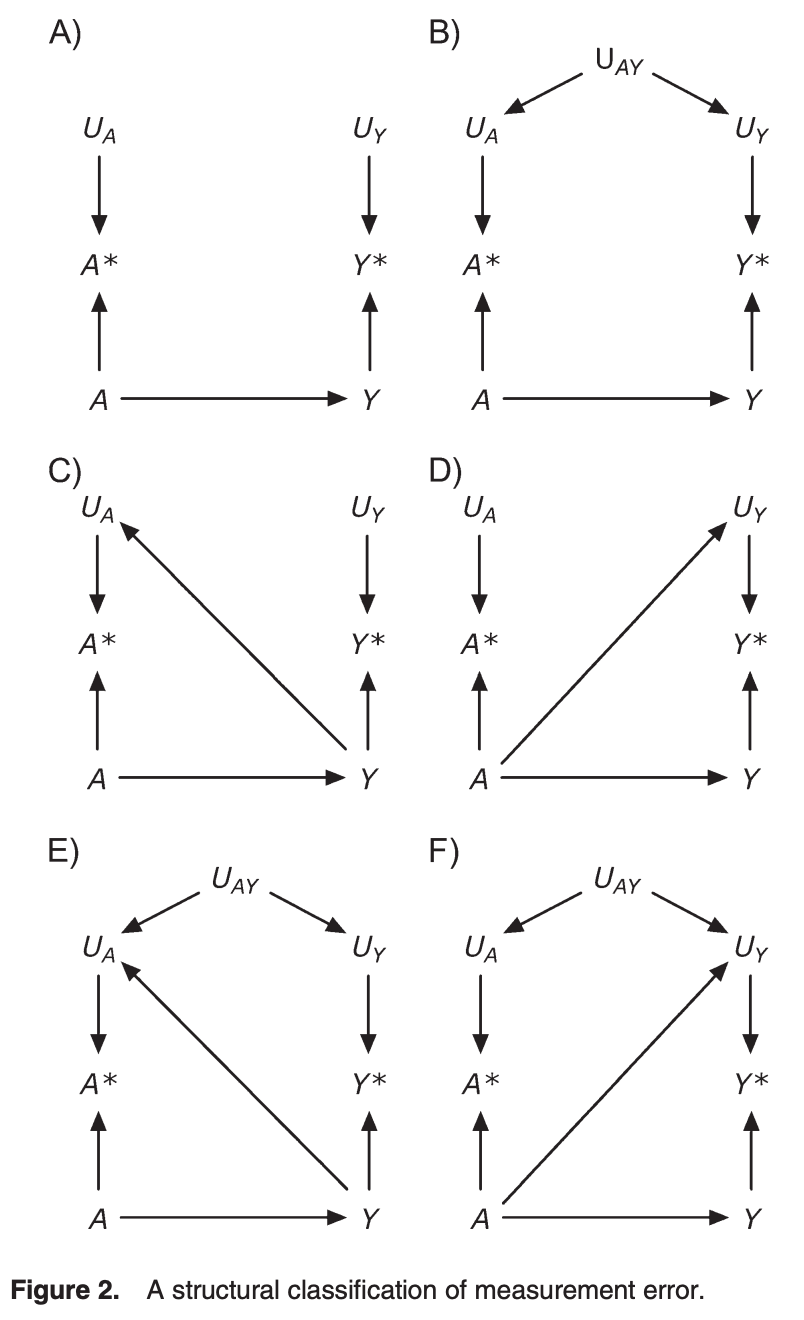
\includegraphics[height = .8\textheight]{figures/hc_fig2}

\end{frame}


\begin{frame}
Hern\'an \& Cole illustration: \vskip .2in
Does body mass index (BMI) affect health outcomes?
\end{frame}

% Note: My usual canvas scale is a bit confused in this frame
\begin{frame}
\begin{tikzpicture}[x = \textwidth, y = .8\textheight]
\node at (0,0) {};
\node at (1,1.3) {};
\node[anchor = north west, align = left, font = \small] (setting) at (0,1.2) {Weight $W$ and height $H$ affect the risk of a condition $A$\\which affects a health outcome $Y$}; 
\pause
\node[anchor = north west, align = left, font = \small] (setting2) at (setting.south west) {Body Mass Index (BMI) is a function\\of measured weight $W^*$ and height $H^*$};
\pause
\node[anchor = north west, align = left, font = \small] (question) at (setting2.south west) {Does BMI affect $Y$?};
\pause
\node (w) at (.15, .35) {$W$};
\node (a) at (.3, .35) {$A$};
\node (h) at (.45, .35) {$H$};
\node (y) at (.7, .35) {$Y$};
\draw[->, thick] (w) -- (a);
\draw[->, thick] (h) -- (a);
\draw[->, thick] (a) to[bend right] (y);
\pause
\node (uw) at (.15, .65) {$U_W$};
\node (uwh) at (.3, .8) {$U_{WH}$};
\node (uh) at (.45, .65) {$U_{H}$};
\node (wstar) at (.15, .5) {$W^*$};
\node (hstar) at (.45, .5) {$H^*$};
\node (ystar) at (.7, .5) {$Y^*$};
\node (uy) at (.7, .65) {$U_Y$};
\draw[->, thick] (uwh) -- (uw);
\draw[->, thick] (uwh) -- (uh);
\draw[->, thick] (uw) -- (wstar);
\draw[->, thick] (uh) -- (hstar);
\draw[->, thick] (w) -- (wstar);
\draw[->, thick] (h) -- (hstar);
\draw[->, thick] (y) -- (ystar);
\draw[->, thick] (uy) -- (ystar);
\pause
\node (bmistar) at (.3, .5) {$\text{BMI}^*$};
\draw[->, thick] (wstar) -- (bmistar);
\draw[->, thick] (hstar) -- (bmistar);
\pause
\node[anchor = north west, align = left, font = \small] at (0,.2) {No. There is no causal path.};
\end{tikzpicture}
\end{frame}

\begin{frame}{Examples to discuss}

\bref{https://tinyurl.com/MeasurementExercise}{tinyurl.com/MeasurementExercise}

\end{frame}

\goalsframe


\begin{frame}{Let me know what you are thinking}

\begin{huge} \bref{https://tinyurl.com/CausalQuestions}{tinyurl.com/CausalQuestions} \end{huge}
\vskip .7in

Office hours TTh 11am-12pm and at \bref{https://calendly.com/ianlundberg/office-hours}{calendly.com/ianlundberg/office-hours}\\Come say hi!

\end{frame}


\end{document}
